\newpage
\section{n-Body GPU computations and streaming}

In this exercise we limited our GPUs memory to 4MB and used a particle number of 512k which comes out to about 16MB for an assumed 32 bytes per particle, which leaves some room for data overhead. The code was implemented using the host memory as a swap space. We firstly load a batch of target particles (positions and velocities), i.e. those onto which forces will be accumulated. We then load batches of source particles (only positions) and accumulate forces from those onto our target particles, until the target particles have a full velocity update and we can update their positions. We then load the next batch of target particles and repeat.\\

This algorithm is actually quite similar to the tiled approach we already use in our optimized kernel calculation. The difference being that the kernel assigns all target particles it is served a thread and only further subdivides the source particles into smaller tiles due to exploit shared memory. In our course grained algorithm both target and source particles have to be batched due to the global memory constraints we imposed. \\

We can additionally overlap some parts of communications and computations using streaming. For example while the position update is being conducted on the target particles we can already write back their velocities to the host. We can also load the target and source particles in parallel. The amount of parallelism we can conduct, at least in our implementation is limited, since both data loads and computations mostly depend on each other and thus cannot be parallelised. \\

The small effect of streaming can be seen in our results (picture). It only leads to a very small speedup, especially at smaller segment sizes, over our non-streamed version (using only stream \#0). \\
\begin{figure}[h]
    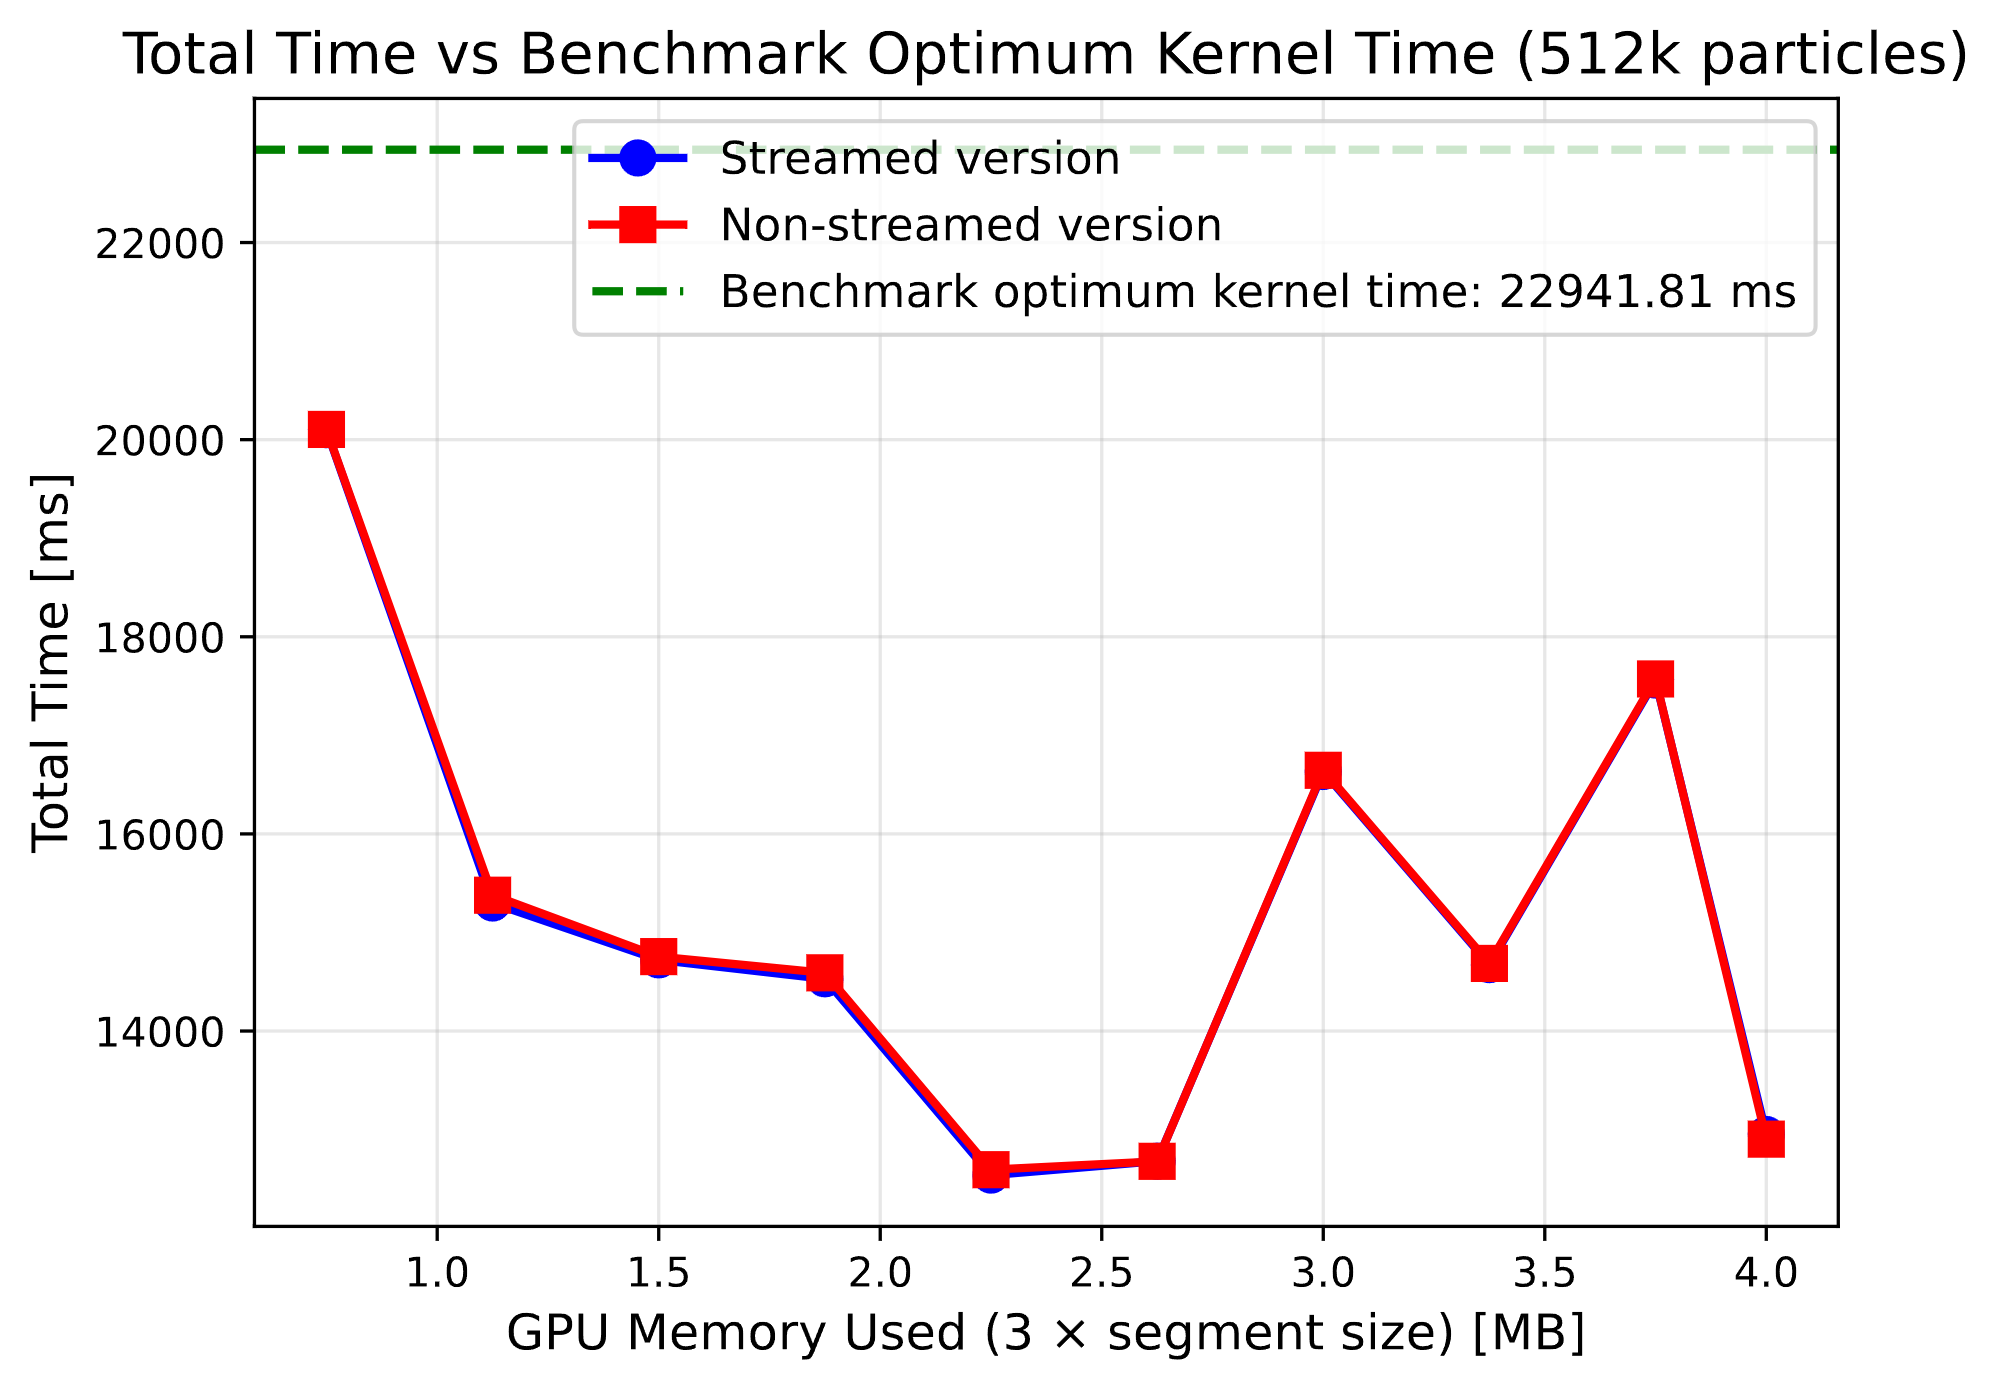
\includegraphics[width=1.0\textwidth]{Ex7_3_nbody_vs_benchmark_kernel.png}
    \caption{Total Time vs Benchmark Optimum Kernel Time by 512k particels}
    \label{fig:Total_vs_OptimumKernel}
\end{figure}
In our implementation we are using three streams, although by using even more fine grained data accesses (i.e. loading and computing two source particle batches simultaneously) could potentially increase the gain from streaming. This would however also increase computational overhead, as we would have to sum up the velocity updates from both batches before we update the velocities of the target particles. This would have to be tested separately in practice. \\

The surprising finding is that our “limited” version is much faster than our optimized benchmark (at a particle size of 512k), with or without streaming. This is likely due the large particle number being much more efficiently processed when it is batched. Without batching one huge kernel has to be launched at once to process all the particles and here we can reduce its overhead by subdividing it into many smaller kernel launches. This improvement seems to dominate even though we move much more data between device and host, which makes sense as  the kernel time dominated the h2d and d2h time already previously. At this particle number the improvement from our optimized version over the benchmark drops to 1.07x (only looking at kernel time)(picture \ref{fig:Speedup_vs_nonOptimized_512k}). The maximum speedup (with a concurrent memory usage of ~2MB on the GPU) is  1.95x (using streams) and 1.94x (without streams). The average is 1.65x (using streams) and 1.64x (without streams). \\
\begin{figure}[h]
    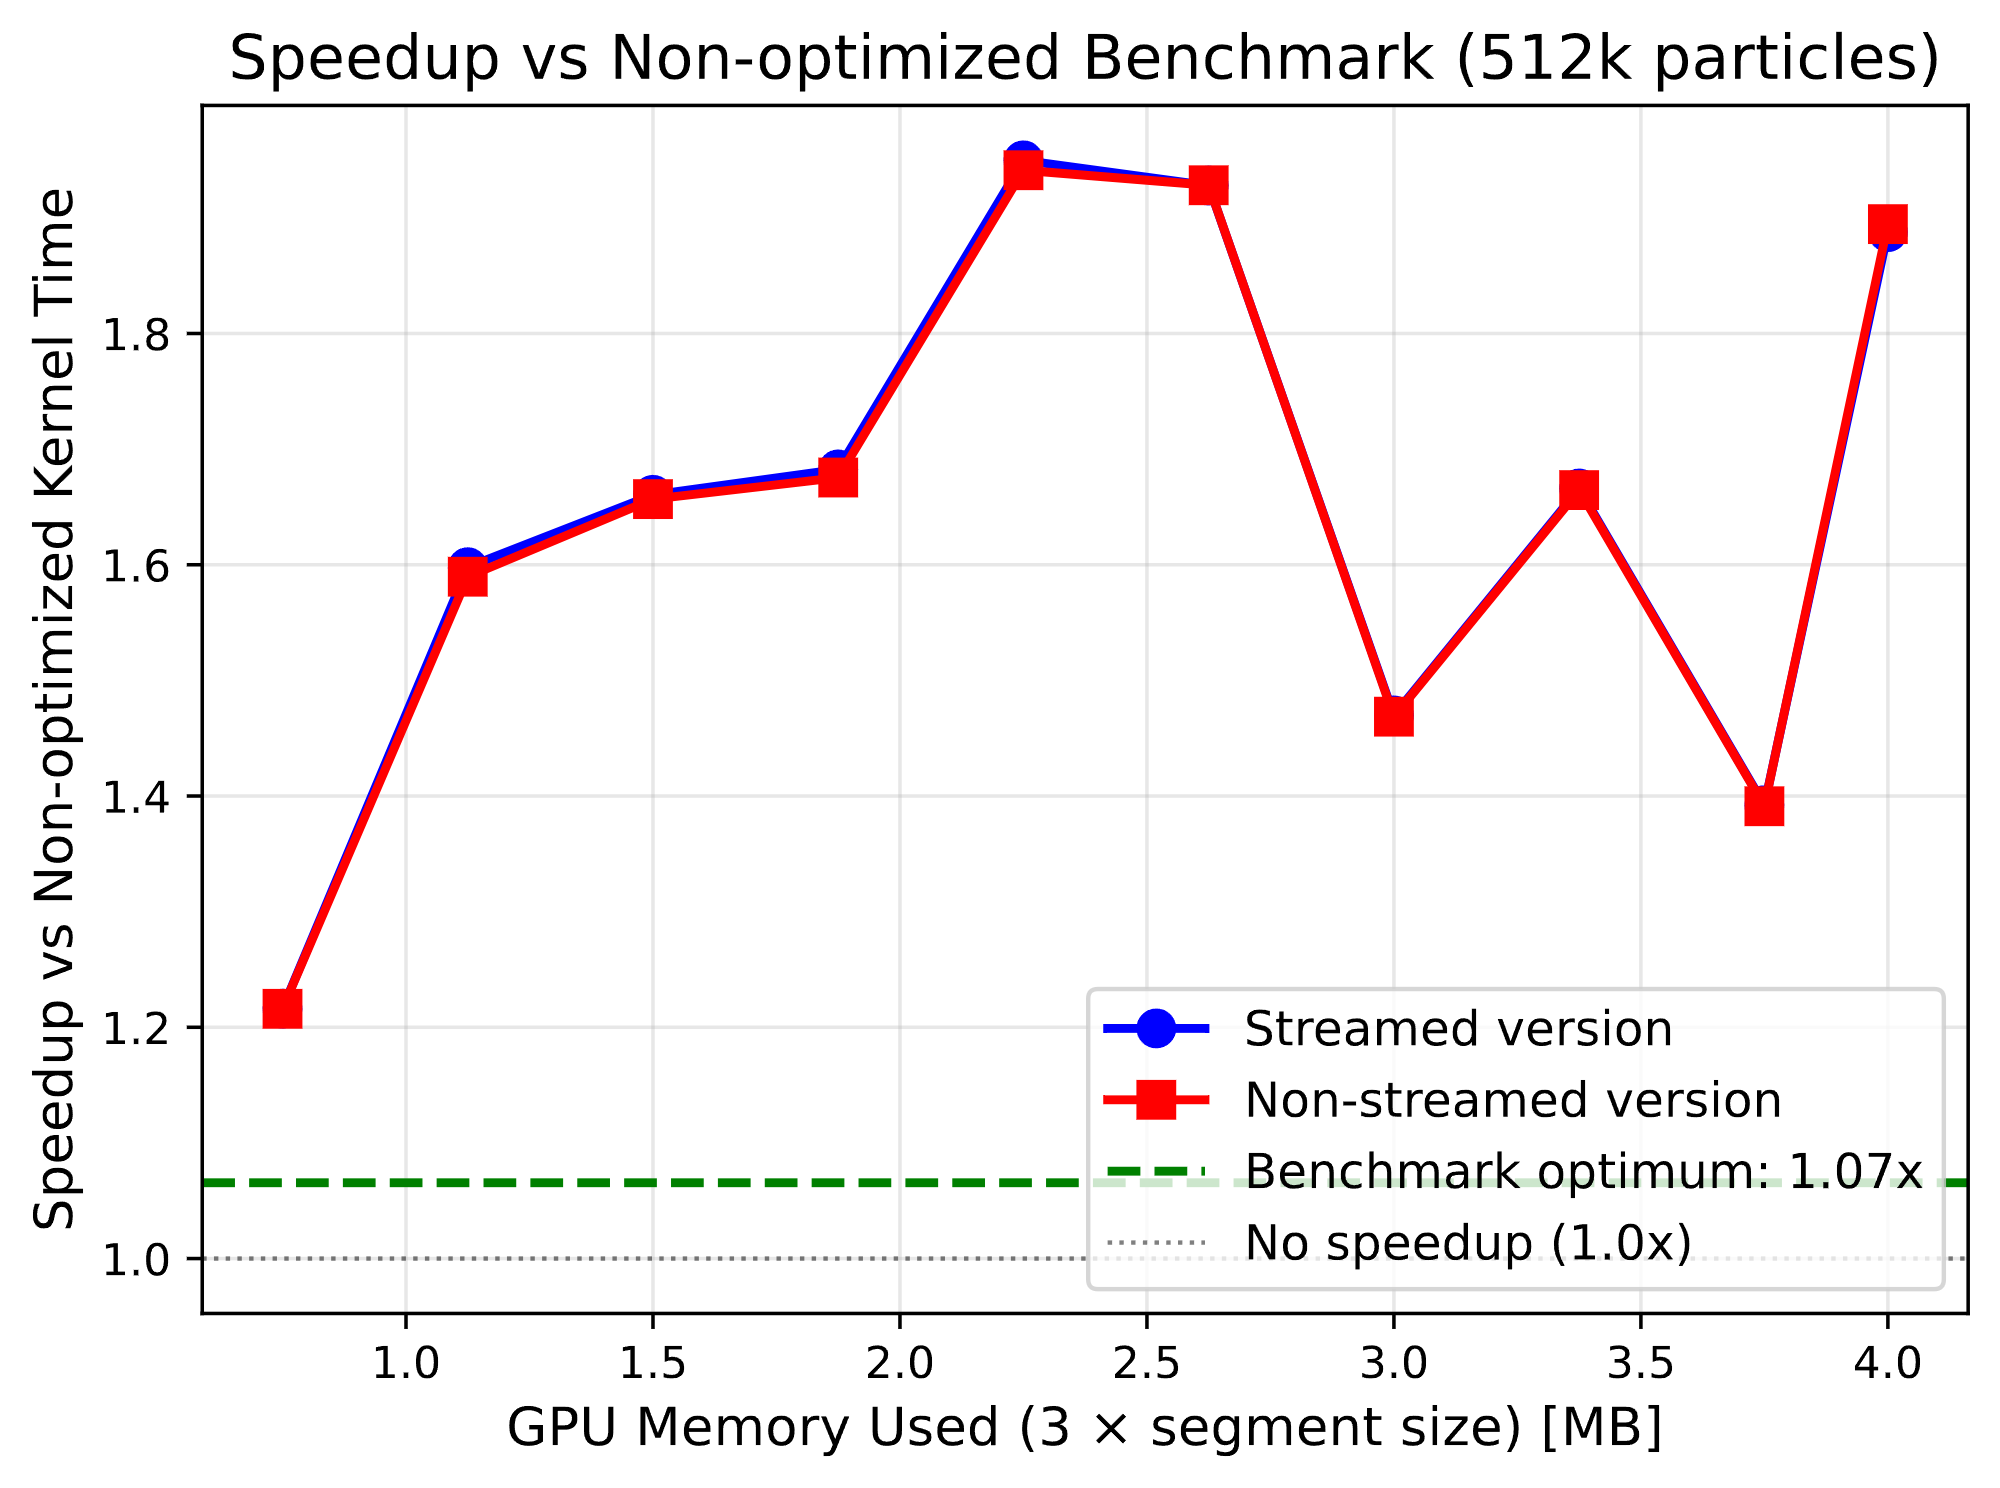
\includegraphics[width=1.0\textwidth]{Ex7_3_nbody_speedup_vs_nonopt_benchmark.png}
    \caption{Speedup vs Non-optimized Benchmark 512k particels}
    \label{fig:Speedup_vs_nonOptimized_512k}
\end{figure}
For different segment sizes we get a different total memory usage on the GPU and also increase the size of kernels launched. We see an increase up until around 2MB memory used, likely because the lower data movement and fewer kernels launched (less launch overhead) is faster. After that we see a decrease around 3MB, likely because the particle number doesn't match well with the segment size and we launch additional kernels for only a few leftover particles. We then see another increase around the maximum 4MB almost back to what we saw at 2MB. As we further increase the segment size we would eventually expect a drop down to the speed of our “optimized” version as the overhead from launching very large kernels would start to dominate.